% Chapter Name
\chapter{\sc Novel Layered Materials Studied with LEEM/LEED-I(V)}
\label{ch:Novel Layered Materials Studied with LEEM/LEED-I(V)}

The study of the fundamental properties of materials and their applications has long been the driving factor in major technological advancements. Applications of novel materials are abundant in areas of research such as sustainable energy sources, healthcare technology, energy efficient transportation, and high speed computing devices \cite{novel-materials}. While not all problems faced by modern society will have a technological solution, it is safe to say that research and innovation in materials science will be crucial to the development and adaptation of many answers to these challenges.

The ability to manipulate and grow materials at the nanoscale has already enabled development of numerous technological advances based on nanotechnology. A wide range of applications from medicine to electronics have been demonstrated using nanoscale materials \cite{nanocancer, energystoragematerials}. The discovery of graphene demonstrated that carbon can be used for nanoscale devices in solid form ranging from zero to three dimensions and furthermore proved that the two-dimensional solid form was not prohibited. However, this discovery also lead to an explosion of research into other materials beyond graphene, which are also stable in two-dimensional form. Given that many new materials have been discovered to be stable in single layer or two-dimensional form, it should be expected that in the future nanotechnology will encompass a wide variety of materials beyond carbon \cite{2d-atlas}.

Many of the currently explored 2D materials posses unique layer dependent electronic properties \cite{2D-TMDs}. Furthermore, single layer and 2D materials span the configuration space of electronic structure from traditional metals, semiconductors, and insulators to more exotic types of materials such as Weyl semimetals, topological insulators, and novel magnetic materials \cite{2d-atlas}. Thus it may be possible in the future to harness the properties of many 2D materials and combine them into devices based on layered heterostructures.

Before devices and new technology can be generated from novel 2D materials, the material properties must be studied at the atomic scale. While many characterization techniques are useful for providing three dimensional structural information for bulk phase materials, the study of the structure of materials in 2D form requires highly surface sensitive probes. Furthermore, given that many current 2D materials are exfoliated into small flakes as opposed to grown via MBE, their characterization requires a probe that can be localized to the micrometer scale and below while also remaining non-destructive. This combination of requirements dramatically reduces the number of possible tools suited for the task.

Here I present a brief overview of the study of two-dimensional materials using LEEM and $\mu$-LEED to analyze the surface structure with {\aa}ngstr\"{o}m level precision. My initial work developing software to analyze LEEM data from our experiments on polymorphic graphene proved immensely useful in a more general sense to analyze both LEEM and LEED \textit{I(V)} data sets from a wide array of surface science experiments concerning the surface structure determination of 2D materials. More information on these studies including their experimental setup as well as corresponding computational and theoretical work can be found in their associated publications as well as the thesis work of my colleague, Zhongwei Dai.


\section{Molybdenum Disulfide}

Molybdenum disulfide belongs to a class of materials known as transition metal dichalcogenides (TMDs). These materials have the formula MX$_2$ where M is a transition metal cation and X is a chalcogen anion; chalcogen atoms fall under group 16 in the periodic table of elements. The molybdenum disulfide bulk crystal structure is composed of sets of layers three atoms in thickness whereby a molybdenum atom is sandwiched between two sulfur atoms. These individual three atom layers are referred to as sandwich layers. One unit cell of bulk MoS$_2$ contains atoms from two such layers consisting of two molybdenum atoms and four sulfur atoms. The sandwich layers of MoS$_2$ are characterized by strong intra-layer bonding and weak inter-layer bonds, which makes the material similar to graphite. As a result, MoS$_2$ also sees use as a lubricant due to the ease at which the sandwich layers can slide against one another. Similar to graphite, the layers of MoS$_2$ can be exfoliated from bulk crystals to form flakes of few layer thickness. Flake thickness can be measured with a variety of tools such as AFM, Raman spectroscopy, and potentially LEEM-\textit{I(V)}.

In bulk form, MoS$_2$ is an indirect gap semiconductor with a band gap of roughly 1.23 eV \cite{MoS2BulkGap}. The lowest direct gap in bulk MoS$_2$ has a larger band gap of nearly 1.8 eV \cite{TMD-bandgaps-ARPES}. However, it has been shown that as the number of layers is reduced from bulk towards a 2D material, MoS$_2$, like other TMDs, undergoes a band gap transition from indirect to direct gap \cite{Mos2GapTransition}. Since the band gap of MoS$_2$ matches well with the solar spectrum, it sees use as an electrode in Photo-electrical-chemical cells \cite{mos2-surfsci}.

Molybdenum disulfide has a variety of polytypes exhibiting different structural configurations, with the 2H polytype is the most stable configuration \cite{mos2-surfsci}. In order to determine the surface structure of this polytype with high resolution, a $\mu$-LEED-\textit{I(V)} study was carried out at Brookhaven National Lab's Center for Functional Nanomaterials. The experimental data was analyzed using the PLEASE software package to extract \textit{I(V)} curves from the (0,0) beam and all first order diffraction beams, as shown in Fig \ref{fig:BulkMoS2}. For each reflected or diffracted beam, the background intensity was also subtracted to improve results. Finally, using dynamical electron multiple scattering calculations, computationally generated \textit{I(V)} curves were matched to the experimental data by optimizing the surface structure parameters such as layer spacing between MoS$_2$ sandwich layers. Detailed information on the surface structure parameters of bulk and monolayer MoS$_2$, and the deviation from the bulk structure can be found in the associated publication \cite{mos2-surfsci}.

\begin{figure}
    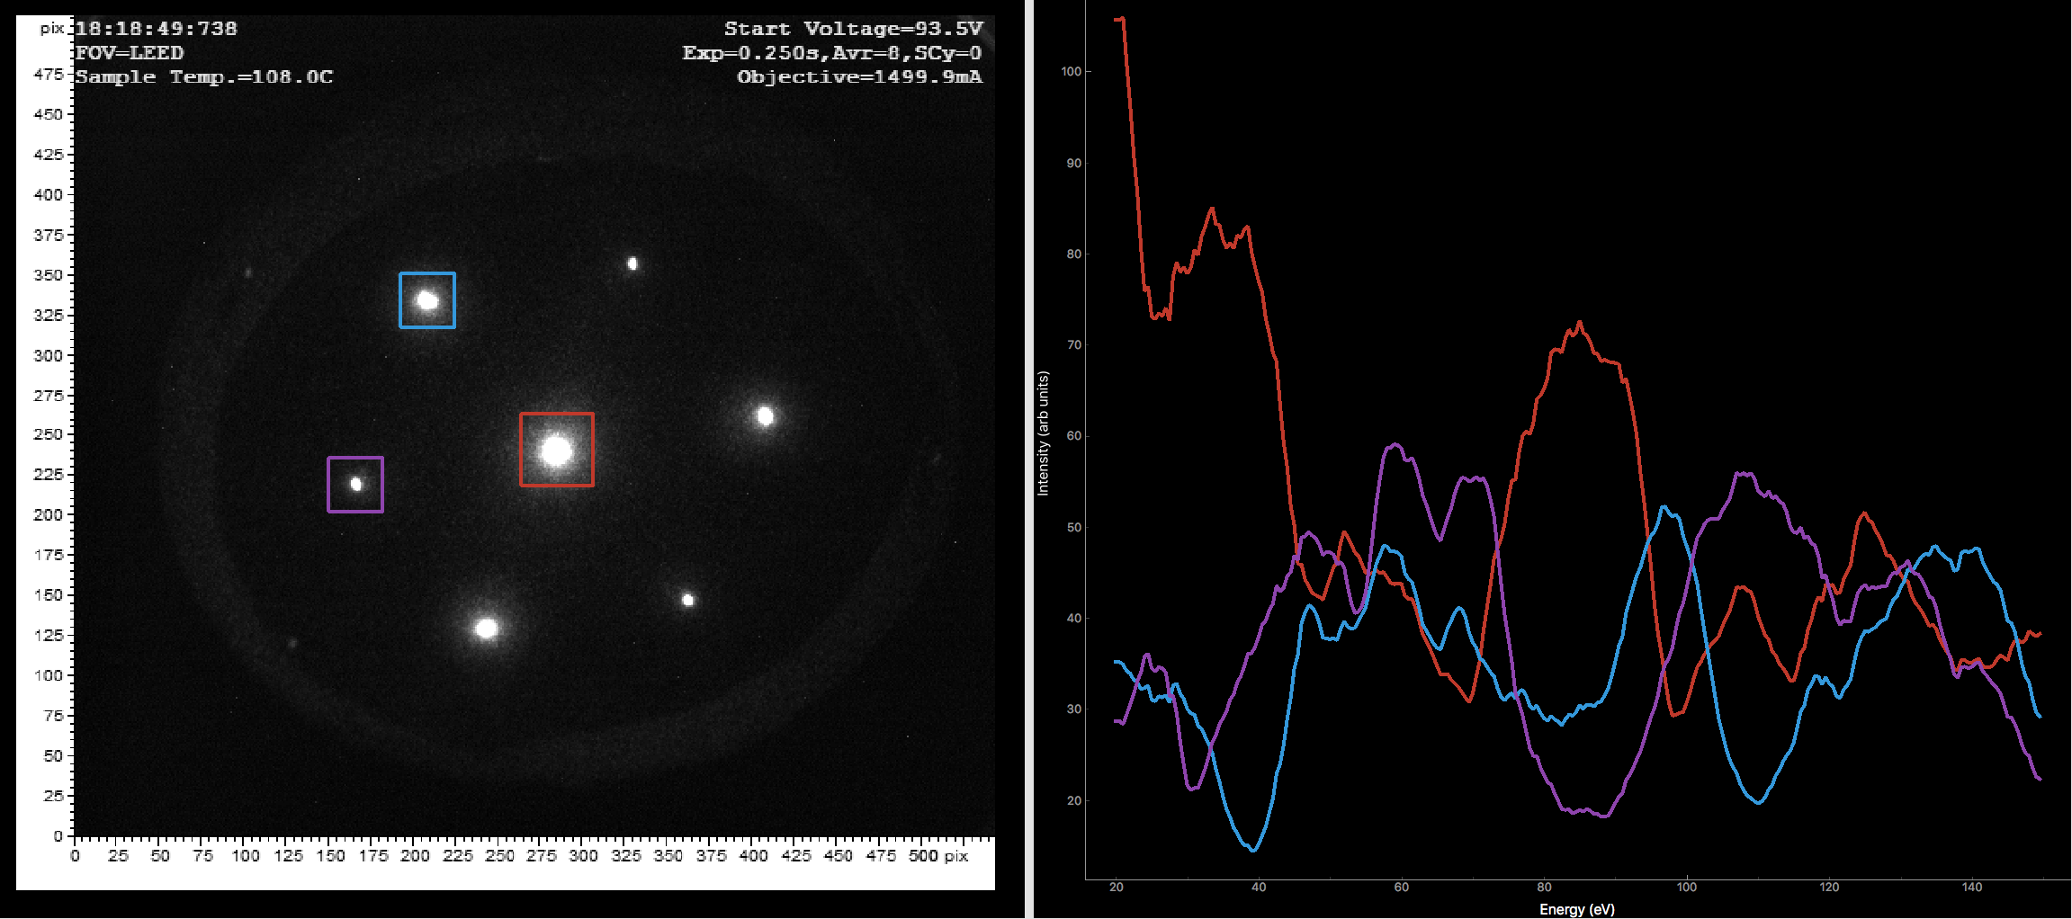
\includegraphics[scale=0.46]{./figs/BulkMoS2-LEED-IV-150.png}
    \caption{LEED-I(V) data set for bulk MoS$_2$ collected at the Brookhaven National Laboratory Center for Functional Nanomaterials. I(V) curves extracted using the PLEASE software package are shown to the left for the (00), (10), and (01) beams. When comparing the experimental data to computationally generated I(V) curves, all symmetric first order beams were averaged together for better results.
    }
    \label{fig:BulkMoS2}
\end{figure}

\section{Black Phosphorous}
Similar to carbon, phosphorus is an element with a wide variety of allotropes. The most common allotropes of phosphorus are distinguished by their color and so named: red, white, violet and black. The different allotropes of phosphorus are also distinguished by their crystal structures. Black phosphorus is a relatively stable allotrope and its bulk form has a crystal structure similar to graphite with the main difference being the pronounced puckering of the hexagonal structure. While the bulk form was originally synthesized in 1914, nearly 100 years later it was found that similar to graphene and TMDs such as MoS$_2$, black phosphorous can be exfoliated into flakes of few layers \cite{bp-ren}.


However, staunchly different from graphene, the black phosphorus surface is highly reactive at ambient conditions and readily oxidizes. Thus, when studying the structure and properties of BP, great care must be taken to exfoliate samples under an inert gas atmosphere \cite{BP-layers-gap}. The electronic and optical properties of black phosphorus have been shown to strongly depend on the layer thickness \cite{BP-layers-gap}. The band gap decreases with increasing layer number, however, unlike make TMDs, black phosphorus does not undergo a transition from direct to indirect band gap or vice versa. In bulk form, BP has a relatively low bandgap of 0.35 eV. The bandgaps of monolayer, bilayer, and trilayer BP, encapsulated between insulating hexagonal boron nitride (h-BN) and a sapphire substrate, are reported to be 1.73 eV, 1.15 eV, and 0.83 eV respectively \cite{BP-layers-gap}. Thus, careful control of the thickness of BP allows highly tailored electronic properties.


As previously mentioned, black phosphorus has a puckered hexagonal lattice with atoms lying in two planes. Ideally the atoms within each plane lie perfectly flat with no out of plane distortion. However, some surface studies have identified a surface buckling that disrupts the ideal lattice structure. STM investigations of the surface structure of black phosphorus reveal an apparent height difference in the surface atoms, however a quantitative measurement of the buckling magnitude was somewhat difficult and estimated at 0.02 to 0.03 {\AA} \cite{bp-buckle-stm}. Since STM imaging couples the geometric features to the local electronic density of states, there is not a high degree of confidence in the accuracy for this value of the surface buckling.

Harnessing the ultra high surface sensitivity of $\mu$-LEED-\textit{I(V)}, we have resolved the atomic surface structure of two separate black phosphorus samples with sub-{\aa}ngstr\"{o}m level resolution. The experimental data was collected using the aberration-corrected LEEM system at the Center for Functional Nanomaterials at Brookhaven National Laboratory. One BP sample was cleaved from bulk under UHV conditions before analysis, the second was exfoliated under an inert gas atmosphere before transfer to the LEEM analysis chamber. \textit{I(V)} curves from the experimental data were extracted using the PLEASE software package. The curves were smoothed to lower the amount of noise and finally the local background signal was subtracted from each curve. Comparison of the experimental LEED-\textit{I(V)} data to the computationally generated curves from dynamical electron multiple scattering theory displays a distinct difference between the ideal unbuckled atomic surface structure and the optimized buckled surface structure. The magnitude of the surface buckling found in this study was an order of magnitude higher than previously reported values. Furthermore, analysis of the origin of the buckling using first principles DFT calculations leads to the conclusion that surface defects are the root cause of both the observed buckling as well as the intrinsic p-type doping commonly observed in black phosphorus \cite{rediscovering-BP}. Details on the experimental setup as well as the DFT calculations for the work on the structure of black phosphorus can be found in the thesis work of my colleague, Zhongwei Dai.

\section{Summary}
By harnessing the high spatial resolution, localization, and non-destructive nature of Low-energy Electron Microscopy, combined with the power of dynamic electron multiple scattering modeling, we have resolved the surface structure of many novel layered and two-dimensional materials with sub-{\aa}ngstr\"{o}m resolution. Furthermore, DFT calculations have helped to understand how changes in surface structure can lead to interesting changes in the electronic properties observed in novel materials. Understanding surface reconstructions and their impact on the electronic properties will be beneficial for future work on development of devices based on heterostructures of novel materials.
